\chapter{Neuro-symbolic Reinforcement Learning Model}
\section{Achitecture Overview}

\begin{figure}[htb]
	\centering
	\begin{tikzpicture}[every node/.style={align=center}, node distance=2cm]

		% Nodes
		\node[draw, thick, rectangle, minimum width=2cm, minimum height=1.2cm] (cnn) {CNN};
		\node[draw, thick, rectangle, minimum width=3cm, minimum height=2cm, right=1.5cm of cnn] (structured) {Structured \\ Representation};
		\node[draw, thick, rectangle, minimum width=2cm, minimum height=1.2cm, below=2cm of cnn] (rnn) {RNN};
		\node[draw, thick, rectangle, minimum width=3cm, minimum height=2cm, right=1.5cm of rnn] (symbolic) {Symbolic \\ Reasoning};
		\node[draw, thick, rectangle, minimum width=2cm, minimum height=1.2cm, right=3cm of structured] (actor) {Actor, $\mu$};
		\node[draw, thick, rectangle, minimum width=3cm, minimum height=1.2cm, above=2cm of actor] (environment) {Environment};
		\node[draw, thick, rectangle, minimum width=2cm, minimum height=1.2cm, below=2cm of actor] (critic) {Critic, $Q$};

		% Connecting Arrows
		\draw[->, thick] (cnn.east) -- (structured.west);
		\draw[->, thick] (structured.south) -- (symbolic.north);
		\draw[->, thick] (symbolic.east) -- (critic.west) node[midway, below] (state) {$s_t$, $s_{t+1}$};
		\draw[->, thick] (state.north) |- (actor.west);
		\draw[->, thick] (actor.north) -- (environment.south) node[midway, left] {$a_t$};
		\draw[->, thick] (actor.south) -- (critic.north) node[midway, left] {$a_t$, $a_{t+1}$};
		\draw[-, thick] (environment.west) -- ++(-4, 0) node[above] (invis) {} -- ++(-4, 0) node[above] (invis2) {};
		\draw[->, thick] (invis2.south) -- node[right] {Image} (cnn.north);
		% \draw[->, thick] (invis.south) -- node[right] {Position} (structured.north);

		\draw[->, thick] (rnn.east) -- (symbolic.west);

		% Input and Output Arrows
		\node[left=0.8cm of rnn] (prompt) {Prompt};
		\node[right=0.8cm of critic] (Q) {$Q_{new}$};
		\draw[->, thick] (prompt.east) -- (rnn.west);
		\draw[->, thick] (critic.east) -- (Q.west);

		% Outer Box
		% \draw[dashed] (-3.75, 4.25) rectangle (6, -4.75) node[above left] {NS-CL};
		% \draw[dashed] (6.25, 4.25) rectangle (12.75, -4.75) node[above left] {DDPG};
		\draw[dashed] (-3.75, 4.25) rectangle (6, -5.25) node[above left] {NS-CL};
		\draw[dashed] (6.25, 4.25) rectangle (12.75, -5.25) node[above left] {DDPG};

	\end{tikzpicture}
  \caption{NS-CL with proposed RL adaptation.}
  \label{fig:architecture}
\end{figure}


\section{Computer Vision}
\begin{figure}[htb]
  \centering
  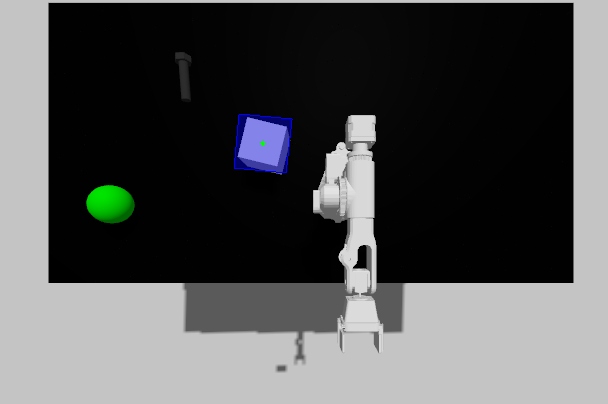
\includegraphics[scale=0.4]{cv}
  \caption{YOLOv8--OBB in Gazebo Simulation}
  \label{fig:cv}
\end{figure}

\subsection{YOLOv8--OBB}
\section{Natural Language Processing}
\section{State Representation}

\begin{table}
	\begin{tiny}
		\begin{center}
			\begin{tabular}{ | m{2cm} | m{2cm}| m{2cm} | m{2cm} | m{3.25cm} |  }
				\hline
				\textbf{Shape} & \textbf{Color $(r, g, b)$} & \textbf{Position $(x,y)$} & \textbf{Rotation $\theta$} & \textbf{Velocity $(v_x, v_y, v_z, \omega)$} \\
				\hline
				J1 & (0, 0, 0) & (0, 0, 0) & 0\textdegree & (0, 0, 0, 0) \\ 
				\hline
				J2 & (0, 0, 0) & (0, 0.1, 0) & 0\textdegree & (0, 0, 0, 0) \\ 
				\hline
				J3 & (0, 0, 0) & (0, 0.2, 0) & 0\textdegree & (0, 0, 0, 0) \\ 
				\hline
				J4 & (0, 0, 0) & (0, 0.4, 0) & 0\textdegree & (0, 0, 0, 0) \\ 
				\hline
				J5 & (0, 0, 0) & (0, 0.4, 0) & 0\textdegree & (0, 0, 0, 0) \\ 
				\hline
				J6 & (0, 0, 0) & (0, 0.4, 0) & 0\textdegree & (0, 0, 0, 0) \\ 
				\hline
				cube & (255, 0, 255) & (0.75, 0.75, 0) & 0\textdegree & (0, 0, 0, 0) \\ 
				\hline
				cylinder & (255, 255, 0) & (-0.25, 1, 0) & 0\textdegree & (0, 0, 0, 0) \\ 
				\hline
				rectangle & (0, 0, 255) & (0.5, 0.5, 0) & 90\textdegree & (0, 0, 0, 0) \\ 
				\hline
				sphere & (0, 255, 0) & (0.6, -0.1, 0) & 0\textdegree & (0, 0, 0, 0) \\ 
				\hline
			\end{tabular}
		\end{center}
	\end{tiny}
	\caption{Example of state observation before symbolic modification.}
	\label{tab:default_state}
\end{table}



\subsection{Symbolic Augmentations}
\begin{table}
	\begin{tiny}
		\begin{center}
			\begin{tabular}{ | m{1cm} | m{1.75cm}| m{2cm} | m{1.5cm} | m{3cm} | m{1cm} | }
				\hline
				\textbf{Label} & \textbf{Color $(r, g, b)$} & \textbf{Position $(x,y)$} & \textbf{Rotation $\theta$} & \textbf{Velocity $(v_x, v_y, v_z, \omega)$} & \textbf{Symbol} \\
				\hline
				J1 & (0, 0, 0) & (0, 0, 0) & 0\textdegree & (0, 0, 0, 0) & null \\ 
				\hline
				J2 & (0, 0, 0) & (0, 0.1, 0) & 0\textdegree & (0, 0, 0, 0) & null\\ 
				\hline
				J3 & (0, 0, 0) & (0, 0.2, 0) & 0\textdegree & (0, 0, 0, 0) & null\\ 
				\hline
				J4 & (0, 0, 0) & (0, 0.4, 0) & 0\textdegree & (0, 0, 0, 0) & null\\ 
				\hline
				J5 & (0, 0, 0) & (0, 0.4, 0) & 0\textdegree & (0, 0, 0, 0) & null \\ 
				\hline
				J6 & (0, 0, 0) & (0, 0.4, 0) & 0\textdegree & (0, 0, 0, 0)& null \\ 
				\hline
				cube & (255, 0, 255) & (0.75, 0.75, 0) & 0\textdegree & (0, 0, 0, 0) & null\\ 
				\hline
				cylinder & (255, 255, 0) & (-0.25, 1, 0) & 0\textdegree & (0, 0, 0, 0) & avoid\\ 
				\hline
				rectangle & (0, 0, 255) & (0.5, 0.5, 0) & 90\textdegree & (0, 0, 0, 0) & move\\ 
				\hline
				sphere & (0, 255, 0) & (0.6, -0.1, 0) & 0\textdegree & (0, 0, 0, 0) & null\\ 
				\hline
				goal & (0, 0, 0) & (-1, 1, 0) & 0\textdegree & (0, 0, 0, 0) & goal\\ 
				\hline
			\end{tabular}
		\end{center}
	\end{tiny}
	\caption{Example of symbolically modified state.}
	\label{tab:symbolic_state}
\end{table}





\section{Reinforcement Learning}
\section{Simulation Environment} \label{se:gazebo_harmonic_robotics_simulator}
    Gazebo is a robotic physics simulator developed by Open Robotics which integrates the ODE physics engine, ORGE rendering engine, and support code for sensor and actuator control integration. This environment leverages Gazebo Harmonic (the latest release of Gazebo at the time of writing) to visually render and simulate the physics of the robotic manipulator and the objects in its environment. 
\subsection{Pick and Place Simulation}
\subsection{Dataset}
The cooresponding dataset used to train the model that can be seen as an extension of the CLEVR dataset [CITATION]-- which instead prompts the agent to act on the objects in the environment.


